\documentclass{article}
\usepackage{clrscode4e}
\usepackage{tikz}
\usetikzlibrary{fit,positioning}
\usepackage{textcomp}
\usepackage{amsmath}
\usepackage{amssymb}

\begin{document}

\section{Overview}
We want to learn how to plan using program induction.
The general idea is that we want a set of compact programs that enable us to sample plans that have a high probability of solving the given tasks.


A \emph{plan} is a list of \emph{actions}.
Each action performs some change of \emph{state}.
Our objective is to find a plan whose actions transform an initial state in to a goal state; there may be many different goal states, or only one.

The learned programs will be either \emph{operators} or \emph{heuristics}.
Operators extend an existing plan by proposing new action sequences.
Heuristics guide the search by rewarding/penalizing certain states.
Given a set of operators and heuristics, a plan may be sampled as follows:

Extend the existing plan by applying all available operators, producing a set of new plans.
Sum the heuristic values for each plan to produce an energy for each plan;
sampling the new plan with probability proportional to the minus exponential of its energy multiplied by an inverse ``temperature'' $\beta=1/T$.
The temperature controls the strength of the heuristic functions:
in the limit as $T\to\infty$, all actions become equally likely, and in the limit as $T\to 0$, the action with the lowest heuristic score is always chosen.

If $\{h_j\}$ are the heuristic functions and $\{(p_i,s_i)\}$ the successor plans and final states to choose from, then
\begin{eqnarray}
\hat{H} &=& \sum_j h_j\mbox{, the ``Heuristic'' or ``Hamiltonian''}\\
Z &=& \sum_i \exp\left( -\frac{\hat{H} s_i}{T} \right)\\
\mbox{P}[(p_i,s_i)] &=& \frac{1}{Z} \exp\left( -\frac{\hat{H} s_i}{T} \right)
\end{eqnarray}

The types of operators and heuristics are:
\begin{eqnarray}
\hat{o}_i \; &:& \; [\mbox{Action}]\times \mbox{State} \to [\mbox{Action}]\\
h_j \; &:& \; \mbox{State} \to \mathbb{R}\cup\{\infty\}
\end{eqnarray}

This model draws from Simon and Newell's models.
According to their models, human planning is sequential, heuristic guided, and doesn't involve (much) backtracking, features which are shared by this sampling procedure.

\section{Generative Model}
The heuristics and actions are drawn from a grammar, $G$, which is drawn from a prior over grammars controlled by the hyperparameter $\lambda$.
Something like $\mbox{P}[G|\lambda]\propto \exp\left(-\lambda |G|\right)$ seems reasonable.
There should also be a prior over the number of heuristics and the number of actions.

We're given $N$ tasks.
For each task a plan $p_i$ is sampled (see section \ref{sec:sample})
which is used to solve task $t_i$.
There is some problem-dependent $P[t_i | p_i]$ which should be higher for plans that do a better job of solving the task, and zero for plans that don't solve the task.
One possibilty is 
\begin{equation}
P[t_i | p_i] \propto \exp\left( -\alpha \mbox{Loss}(t_i,p_i)\right)
\end{equation}
For tower building the loss function is the number of blocks used.
For constructive solid geometry, one possibility is the sum of the $\mbox{L}_2$ norms of the pixel differences between the target image and the rendered image when projected on to various 2D planes.
Or, we could look at the number of differing voxels.

\begin{figure}
\centering
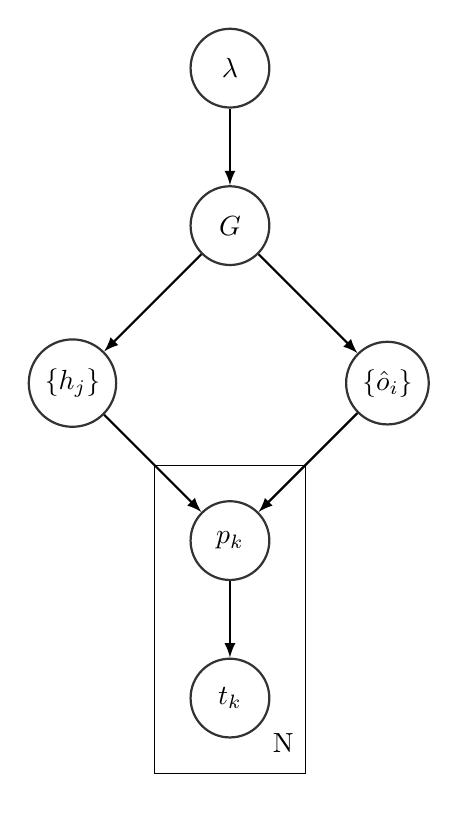
\begin{tikzpicture}
\tikzstyle{main}=[circle, minimum size = 10mm, thick, draw =black!80, node distance = 16mm]
\tikzstyle{connect}=[-latex, thick]
\tikzstyle{box}=[rectangle, draw=black!100]

\node[main, fill = white!100] at (0,2) (lambda)  {$\lambda$ };
\node[main, fill = white!100] at (0, 0) (grammar)  {$G$ };
\node[main, fill = white!100] at (2,-2) (actions) {$\{\hat{o}_i\}$ };
\node[main, fill = white!100] at (-2,-2) (heuristic) {$\{h_j\}$ };
\node[main, fill = white!100] at (0,-4) (psubk) {$p_k$ };
\node[main, fill = white!100] at (0,-6) (tsubk) {$t_k$ };
\path (lambda) edge [connect] (grammar);
\path (grammar) edge [connect] (heuristic);
\path (grammar) edge [connect] (actions);
\path (heuristic) edge [connect] (psubk);
\path (actions) edge [connect] (psubk);
\path (psubk) edge [connect] (tsubk);
\node[rectangle, inner sep=0mm, fit= (psubk) (tsubk),label=below right:N, xshift=-1mm, yshift=-8mm] {};
\node[rectangle, inner sep=4.4mm,draw=black!100, fit= (psubk) (tsubk)] {};
\end{tikzpicture}
\end{figure}


\section{Sampling}\label{sec:sample}
\begin{codebox}
\Procname{$\proc{Sample-Plan}(\{\hat{o}_i\}, \{h_j\}, depth)$}
\li \id{plan} = [ ]
\li \id{state} = \const{initial state}
\li \id{T} = \const{temperature}
\li \textbf{repeat} \id{depth} \textbf{times}\Do
\li \Comment{Get new plans and new states:}
\li \id{p'_i} = \id{\hat{o}_i}(\id{p}, \id{s})
\li \id{s'_i} = \func{Run-Actions}(\id{p'_i}, \id{s})
\li
\li \Comment{Compute energies and partition function:}
\li \id{E_i} = $\sum_j$ \id{h_j}(\id{s'_i})
\li \id{Z} = $\sum_i$ $\exp \left( -E_i / T \right)$
\li
\li \Comment{Sample next action, and then apply it:}
\li \id{i^*} $\sim$ \func{Multinomial}$\left(\frac{1}{Z}\exp(-E_1/T), \frac{1}{Z}\exp(-E_2/T), ...\right)$
\li \id{plan} = \id{plan} $\cdot$ \id{p_{i^*}}
\li \id{state} = \id{s'_{i^*}}
\li 
\li \Comment{Check if goal state is reached:}
\li \If \func{Is-Goal}(\id{state}) \Then
\li \Return \id{plan}, \id{state}
\li \End\End
\li \Comment{Failure to find a plan within depth \emph{depth}:}
\li \Return $\bot$
\end{codebox}


\end{document}

